\documentclass[12pt]{article}
\usepackage{amsmath}
\usepackage{amssymb} %mathbb
\usepackage{graphicx}
\usepackage{hyperref}
\usepackage{gensymb}
\usepackage[latin1]{inputenc}
\usepackage[top=1.0cm,bottom=1.3cm,left=1.0cm,right=1.0cm]{geometry}

\begin{document}

\Large

\begin{center}
Resum\~ao | RUDIN, W.; Real and Complex Analysis; Third Edition
\end{center}

\normalsize

1) Integra\c{c}\~ao em Abstrato

\vspace{3mm}

		\begin{center}
		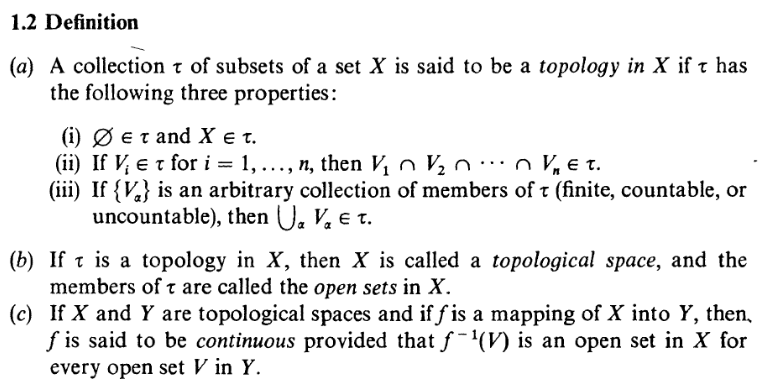
\includegraphics{d1ponto2}
		\end{center}

		\begin{center}
		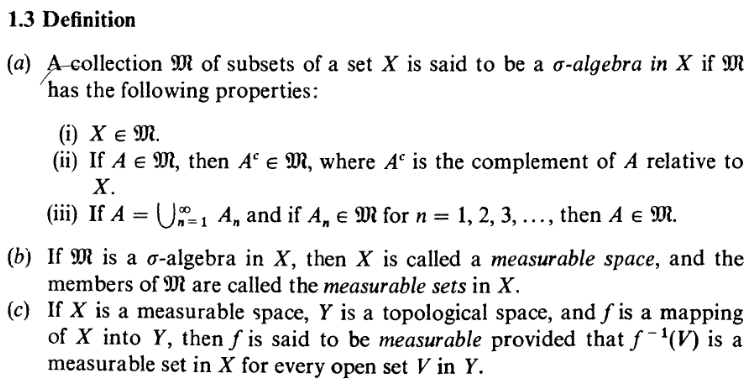
\includegraphics{d1ponto3}
		\end{center}

		\begin{center}
		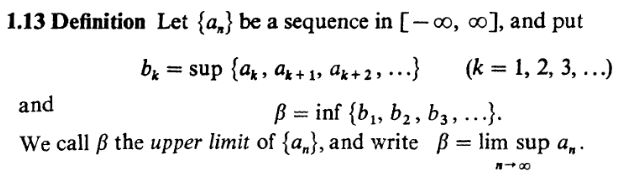
\includegraphics{d1ponto13}
		\end{center}

		\begin{center}
		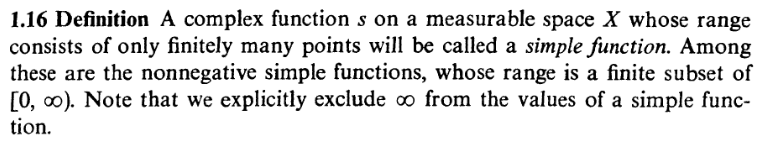
\includegraphics{d1ponto16}
		\end{center}

		\begin{center}
		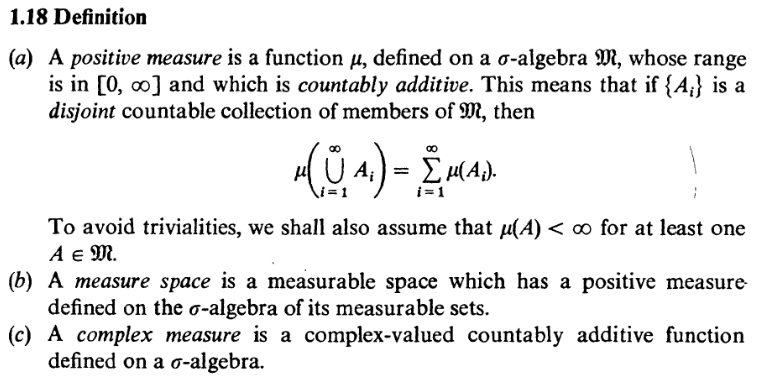
\includegraphics{d1ponto18}
		\end{center}

		\begin{center}
		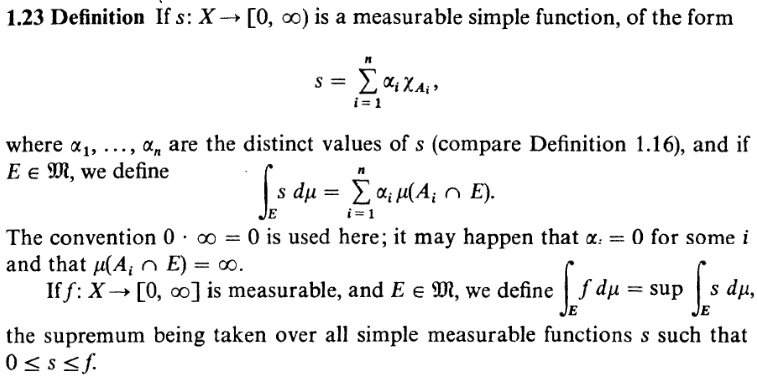
\includegraphics{d1ponto23}
		\end{center}

		\begin{center}
		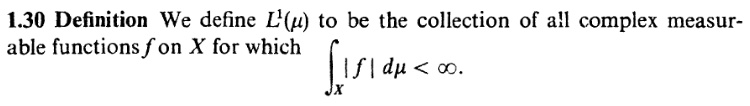
\includegraphics{d1ponto30}
		\end{center}

		\begin{center}
		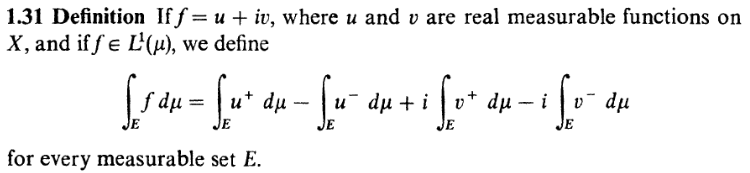
\includegraphics{d1ponto31}
		\end{center}

		\begin{center}
		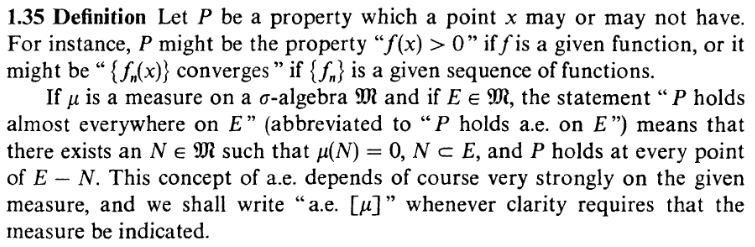
\includegraphics{d1ponto35}
		\end{center}

Lista de teoremas:

		\begin{center}
		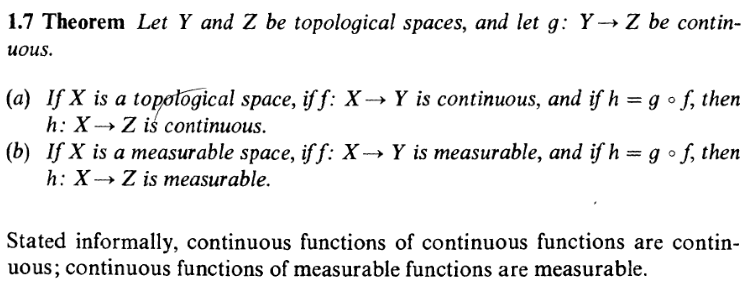
\includegraphics{1ponto7}
		\end{center}

		\begin{center}
		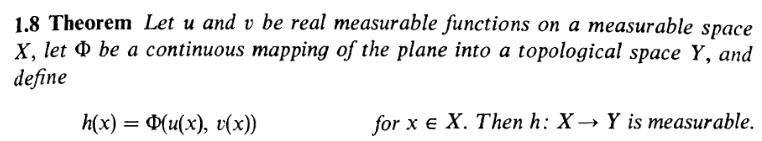
\includegraphics{1ponto8}
		\end{center}

		\begin{center}
		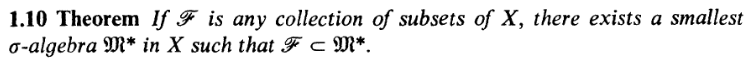
\includegraphics{1ponto10}
		\end{center}

		\begin{center}
		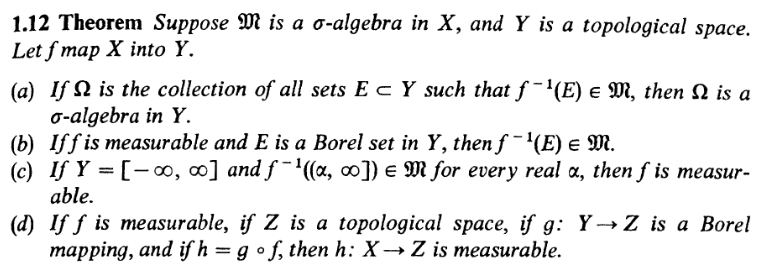
\includegraphics{1ponto12}
		\end{center}

		\begin{center}
		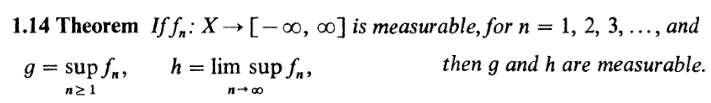
\includegraphics{1ponto14}
		\end{center}

		\begin{center}
		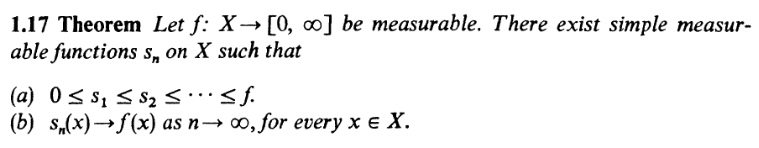
\includegraphics{1ponto17}
		\end{center}

		\begin{center}
		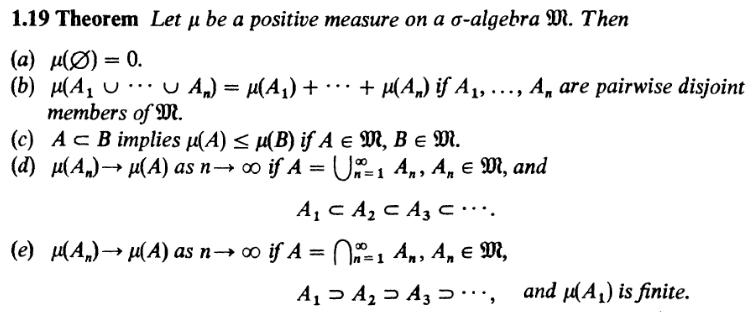
\includegraphics{1ponto19}
		\end{center}

		\begin{center}
		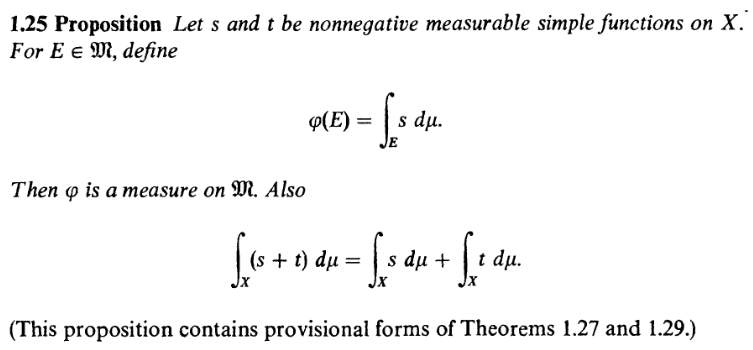
\includegraphics{1ponto25}
		\end{center}

		\begin{center}
		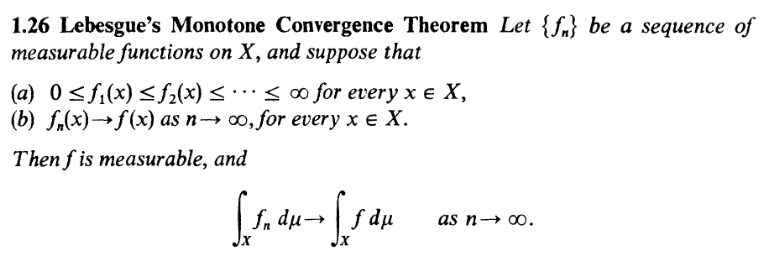
\includegraphics{1ponto26}
		\end{center}

		\begin{center}
		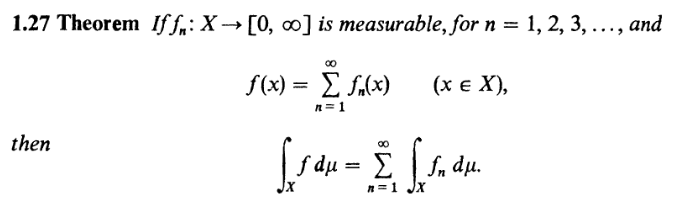
\includegraphics{1ponto27}
		\end{center}

		\begin{center}
		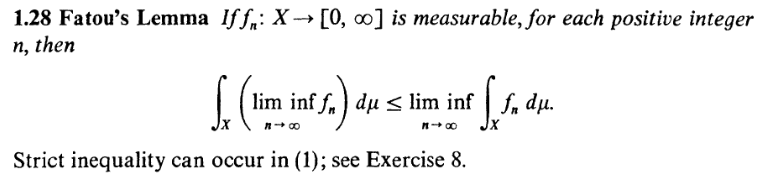
\includegraphics{1ponto28}
		\end{center}

		\begin{center}
		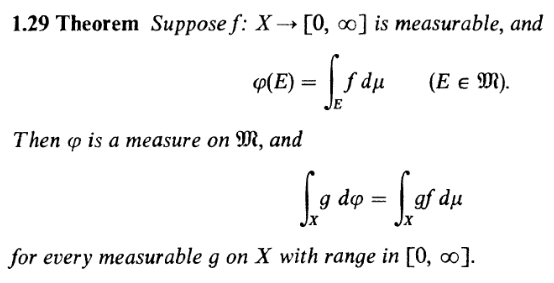
\includegraphics{1ponto29}
		\end{center}

		\begin{center}
		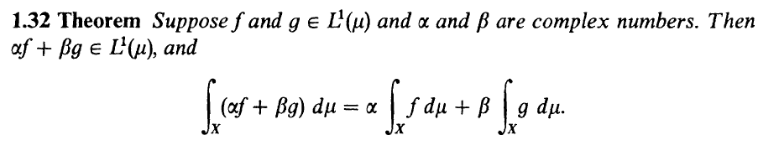
\includegraphics{1ponto32}
		\end{center}

		\begin{center}
		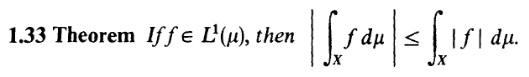
\includegraphics{1ponto33}
		\end{center}

		\begin{center}
		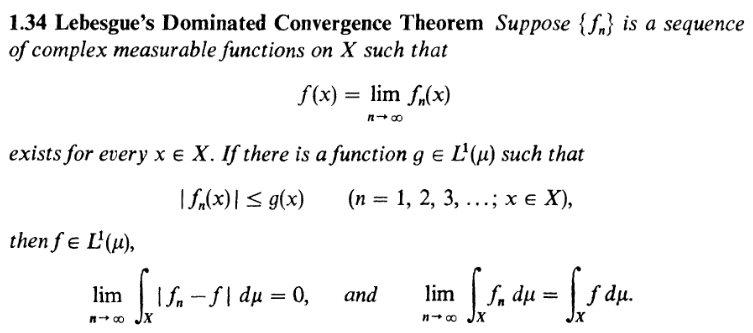
\includegraphics{1ponto34}
		\end{center}

		\begin{center}
		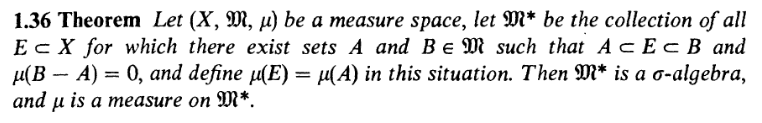
\includegraphics{1ponto36}
		\end{center}

		\begin{center}
		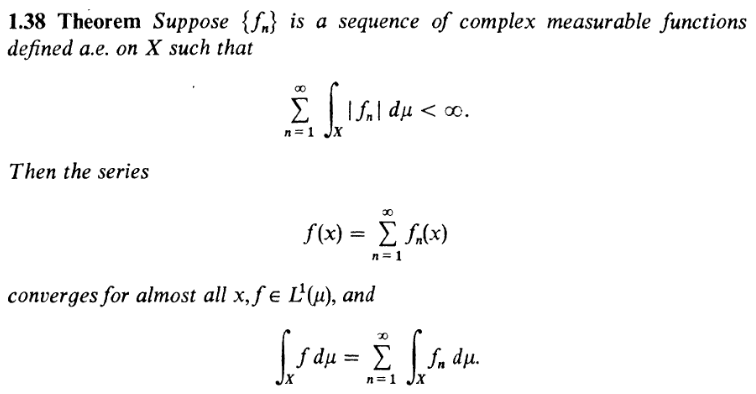
\includegraphics{1ponto38}
		\end{center}

		\begin{center}
		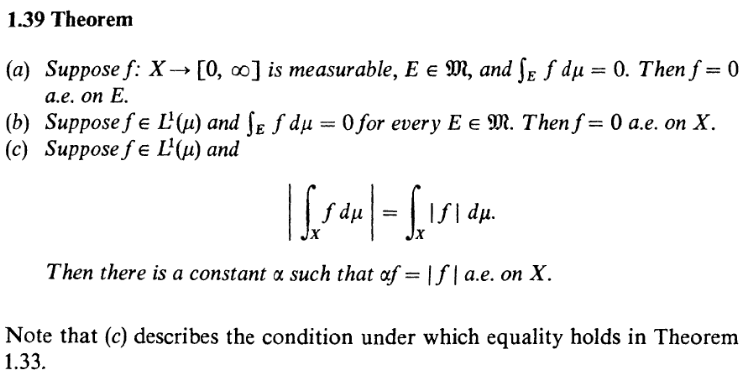
\includegraphics{1ponto39}
		\end{center}

		\begin{center}
		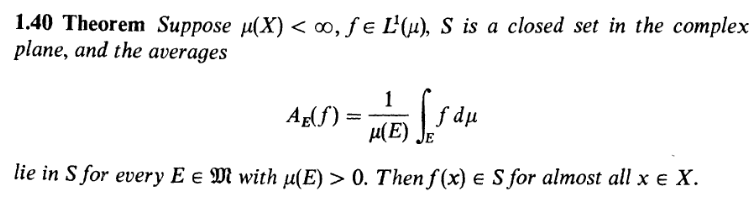
\includegraphics{1ponto40}
		\end{center}

		\begin{center}
		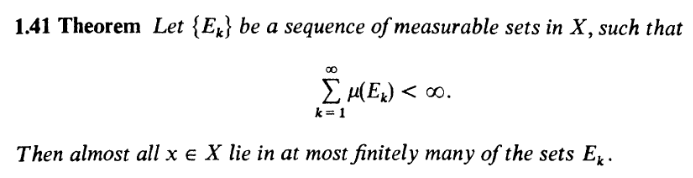
\includegraphics{1ponto41}
		\end{center}

\vspace{3mm}

2) Medidas Borelianas Positivas

\vspace{3mm}

		\begin{center}
		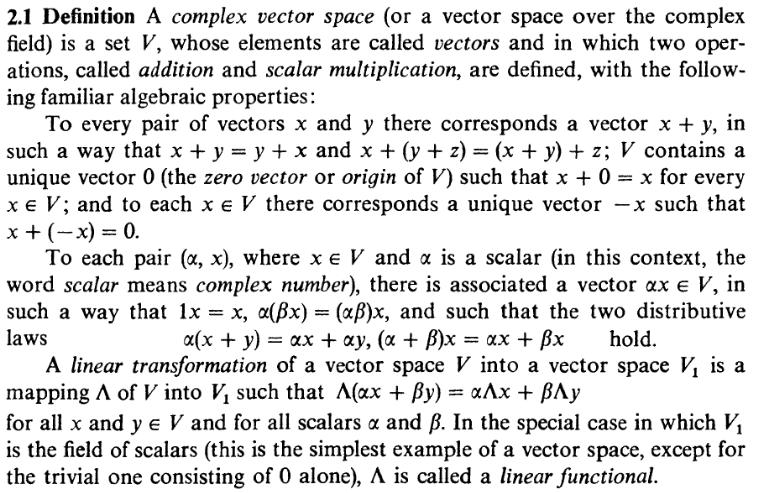
\includegraphics{d2ponto1}
		\end{center}

		\begin{center}
		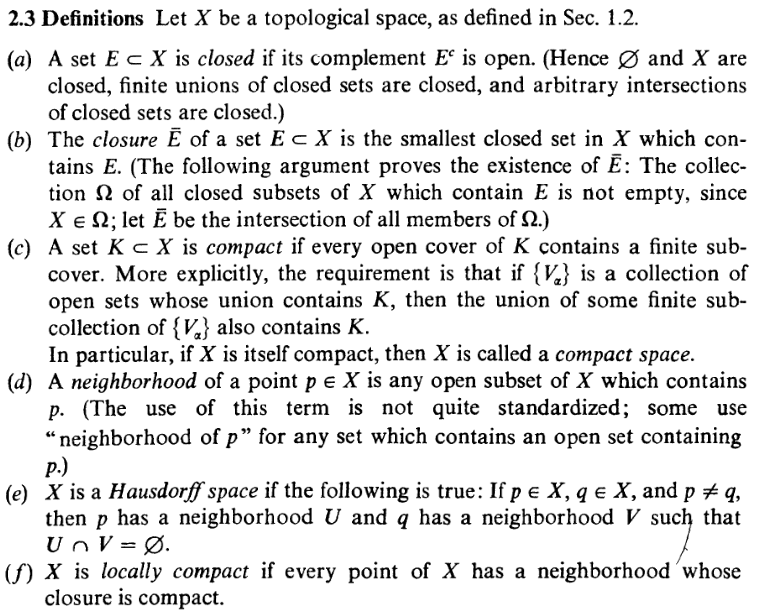
\includegraphics{d2ponto3}
		\end{center}

		\begin{center}
		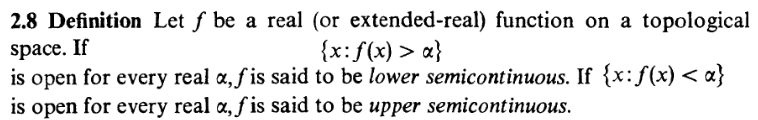
\includegraphics{d2ponto8}
		\end{center}

		\begin{center}
		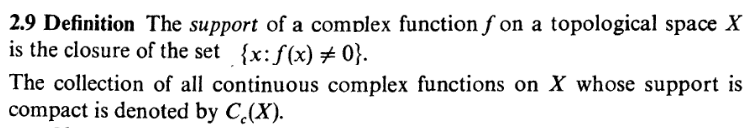
\includegraphics{d2ponto9}
		\end{center}

		\begin{center}
		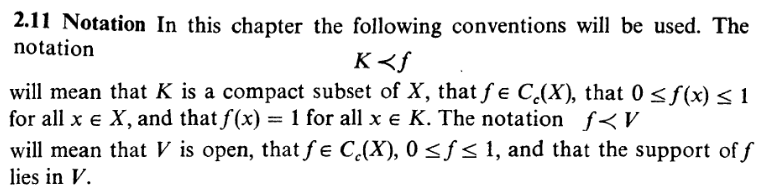
\includegraphics{d2ponto11}
		\end{center}

		\begin{center}
		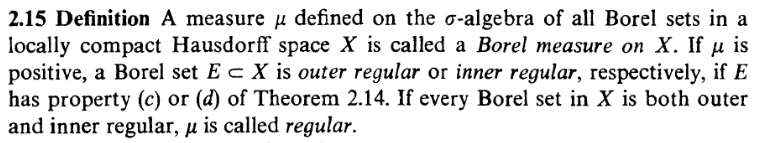
\includegraphics{d2ponto15}
		\end{center}

		\begin{center}
		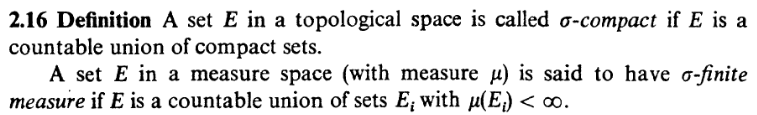
\includegraphics{d2ponto16}
		\end{center}

Lista de teoremas:

		\begin{center}
		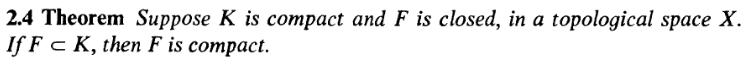
\includegraphics{2ponto4}
		\end{center}

		\begin{center}
		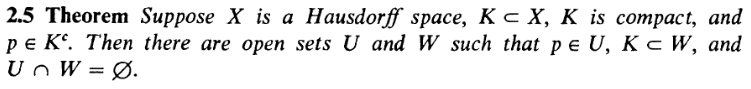
\includegraphics{2ponto5}
		\end{center}

		\begin{center}
		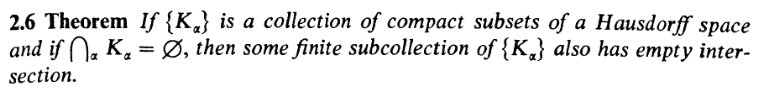
\includegraphics{2ponto6}
		\end{center}

		\begin{center}
		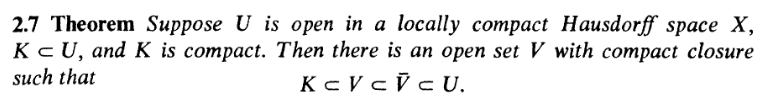
\includegraphics{2ponto7}
		\end{center}

		\begin{center}
		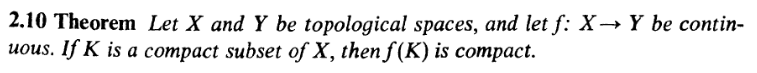
\includegraphics{2ponto10}
		\end{center}

		\begin{center}
		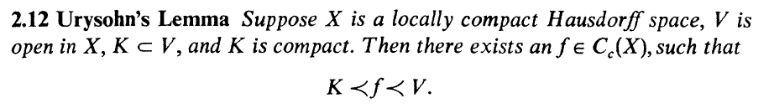
\includegraphics{2ponto12}
		\end{center}

		\begin{center}
		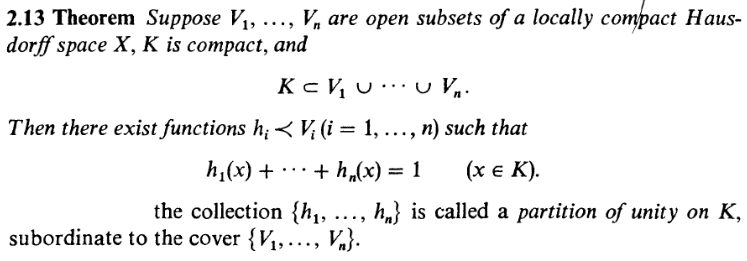
\includegraphics{2ponto13}
		\end{center}

		\begin{center}
		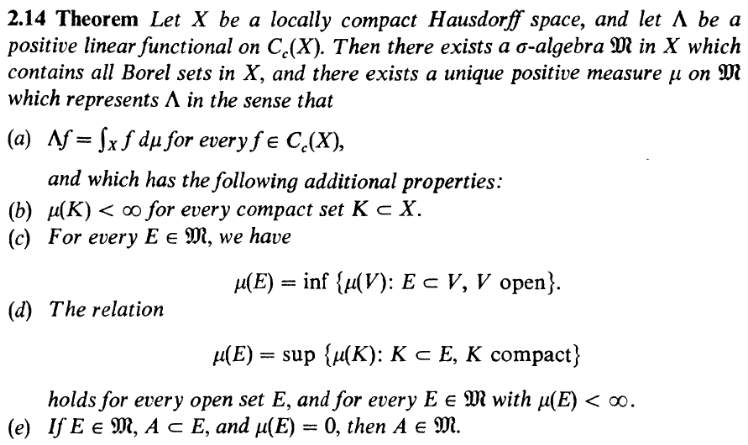
\includegraphics{2ponto14}
		\end{center}

		\begin{center}
		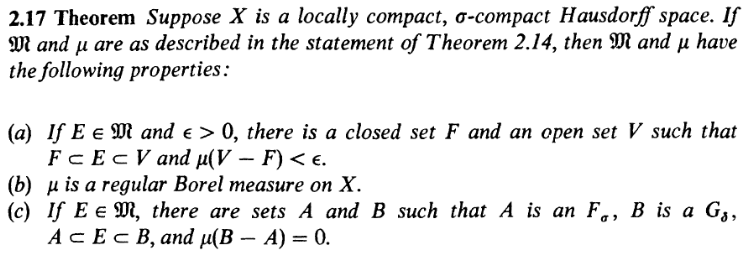
\includegraphics{2ponto17}
		\end{center}

		\begin{center}
		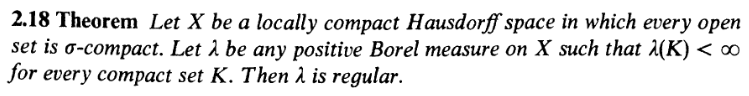
\includegraphics{2ponto18}
		\end{center}

		\begin{center}
		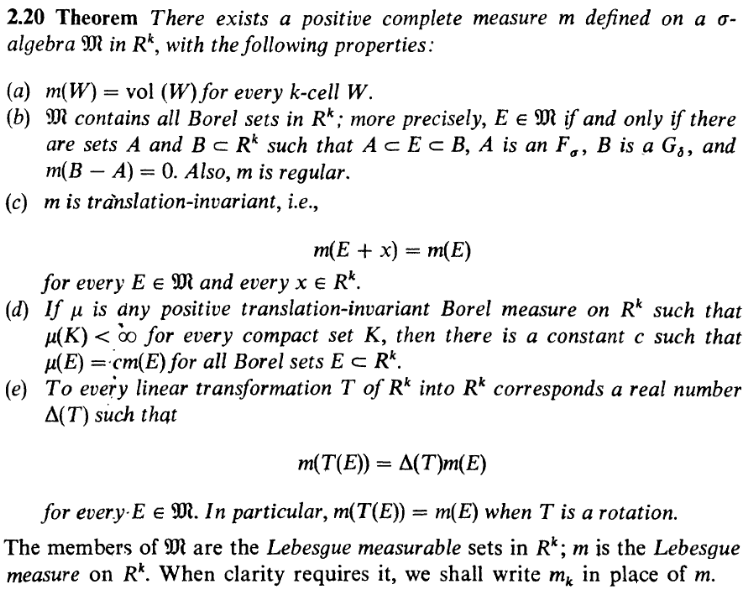
\includegraphics{2ponto20}
		\end{center}

		\begin{center}
		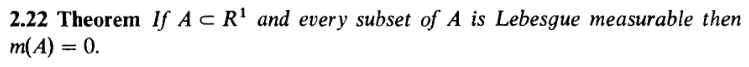
\includegraphics{2ponto22}
		\end{center}

		\begin{center}
		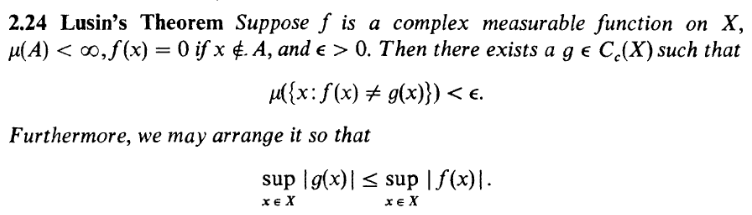
\includegraphics{2ponto24}
		\end{center}

		\begin{center}
		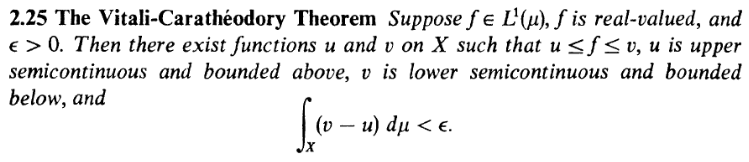
\includegraphics{2ponto25}
		\end{center}

\vspace{3mm}

3) Espa\c{c}os $L^p$

\vspace{3mm}

		\begin{center}
		\includegraphics{d3ponto1}
		\end{center}

		\begin{center}
		\includegraphics{d3ponto4}
		\end{center}

		\begin{center}
		\includegraphics{d3ponto6}
		\end{center}

		\begin{center}
		\includegraphics{d3ponto7}
		\end{center}

		\begin{center}
		\includegraphics{d3ponto16}
		\end{center}

Lista de teoremas:

		\begin{center}
		\includegraphics{3ponto2}
		\end{center}

		\begin{center}
		\includegraphics[scale=0.9]{3ponto3}
		\end{center}

		\begin{center}
		\includegraphics{3ponto5}
		\end{center}

		\begin{center}
		\includegraphics{3ponto8}
		\end{center}

		\begin{center}
		\includegraphics{3ponto9}
		\end{center}

		\begin{center}
		\includegraphics{3ponto11}
		\end{center}

		\begin{center}
		\includegraphics{3ponto12}
		\end{center}

		\begin{center}
		\includegraphics{3ponto13}
		\end{center}

		\begin{center}
		\includegraphics{3ponto14}
		\end{center}

		\begin{center}
		\includegraphics{3ponto17}
		\end{center}

\vspace{3mm}

4) Teoria Elementar de Espa\c{c}os de Hilbert

\vspace{3mm}

		\begin{center}
		\includegraphics{d4ponto1}
		\end{center}

		\begin{center}
		\includegraphics{d4ponto4}
		\end{center}

		\begin{center}
		\includegraphics{d4ponto13}
		\end{center}

		\begin{center}
		\includegraphics{d4ponto23}
		\end{center}

Lista de teoremas:

		\begin{center}
		\includegraphics{4ponto2}
		\end{center}

		\begin{center}
		\includegraphics{4ponto3}
		\end{center}

		\begin{center}
		\includegraphics{4ponto6}
		\end{center}

		\begin{center}
		\includegraphics{4ponto10}
		\end{center}

		\begin{center}
		\includegraphics{4ponto11}
		\end{center}

		\begin{center}
		\includegraphics{4ponto12}
		\end{center}

		\begin{center}
		\includegraphics{4ponto14}
		\end{center}

		\begin{center}
		\includegraphics{4ponto16}
		\end{center}

		\begin{center}
		\includegraphics{4ponto17}
		\end{center}

		\begin{center}
		\includegraphics{4ponto18}
		\end{center}

		\begin{center}
		\includegraphics{4ponto21}
		\end{center}

		\begin{center}
		\includegraphics{4ponto22}
		\end{center}

		\begin{center}
		\includegraphics{4ponto25}
		\end{center}

\vspace{3mm}

5) Exemplos de T\'ecnicas de Espa\c{c}o de Banach

\vspace{3mm}

		\begin{center}
		\includegraphics{d5ponto2}
		\end{center}

		\begin{center}
		\includegraphics{d5ponto3}
		\end{center}

Lista de teoremas:

		\begin{center}
		\includegraphics{5ponto4}
		\end{center}

		\begin{center}
		\includegraphics{5ponto6}
		\end{center}

		\begin{center}
		\includegraphics{5ponto8}
		\end{center}

		\begin{center}
		\includegraphics{5ponto9}
		\end{center}

		\begin{center}
		\includegraphics{5ponto10}
		\end{center}

		\begin{center}
		\includegraphics{5ponto12}
		\end{center}

		\begin{center}
		\includegraphics{5ponto13}
		\end{center}

		\begin{center}
		\includegraphics{5ponto15}
		\end{center}

		\begin{center}
		\includegraphics{5ponto16}
		\end{center}

		\begin{center}
		\includegraphics{5ponto17}
		\end{center}

		\begin{center}
		\includegraphics{5ponto19}
		\end{center}

		\begin{center}
		\includegraphics{5ponto20}
		\end{center}

		\begin{center}
		\includegraphics{5ponto25}
		\end{center}

\vspace{3mm}

6) Medidas Complexas

\vspace{3mm}

		\begin{center}
		\includegraphics{d6ponto7}
		\end{center}

Lista de teoremas:

		\begin{center}
		\includegraphics{6ponto2}
		\end{center}

		\begin{center}
		\includegraphics{6ponto3}
		\end{center}

		\begin{center}
		\includegraphics{6ponto4}
		\end{center}

		\begin{center}
		\includegraphics{6ponto8}
		\end{center}

		\begin{center}
		\includegraphics{6ponto9}
		\end{center}

		\begin{center}
		\includegraphics{6ponto10}
		\end{center}

		\begin{center}
		\includegraphics{6ponto11}
		\end{center}

		\begin{center}
		\includegraphics{6ponto12}
		\end{center}

		\begin{center}
		\includegraphics{6ponto13}
		\end{center}

		\begin{center}
		\includegraphics[scale=0.9]{6ponto14}
		\end{center}

		\begin{center}
		\includegraphics{6ponto16}
		\end{center}

		\begin{center}
		\includegraphics{6ponto19}
		\end{center}

\vspace{3mm}

7) Diferencia\c{c}\~ao

\vspace{3mm}

		\begin{center}
		\includegraphics{d7ponto2}
		\end{center}

		\begin{center}
		\includegraphics{d7ponto5}
		\end{center}

		\begin{center}
		\includegraphics{d7ponto6}
		\end{center}

		\begin{center}
		\includegraphics[scale=0.9]{d7ponto12}
		\end{center}

		\begin{center}
		\includegraphics{d7ponto17}
		\end{center}

		\begin{center}
		\includegraphics{d7ponto22}
		\end{center}

Lista de teoremas:

		\begin{center}
		\includegraphics{7ponto1}
		\end{center}

		\begin{center}
		\includegraphics{7ponto3}
		\end{center}

		\begin{center}
		\includegraphics{7ponto4}
		\end{center}

		\begin{center}
		\includegraphics{7ponto7}
		\end{center}

		\begin{center}
		\includegraphics{7ponto8}
		\end{center}

		\begin{center}
		\includegraphics{7ponto10}
		\end{center}

		\begin{center}
		\includegraphics{7ponto11}
		\end{center}

		\begin{center}
		\includegraphics{7ponto13}
		\end{center}

		\begin{center}
		\includegraphics{7ponto14}
		\end{center}

		\begin{center}
		\includegraphics{7ponto15}
		\end{center}

		\begin{center}
		\includegraphics{7ponto18}
		\end{center}

		\begin{center}
		\includegraphics{7ponto19}
		\end{center}

		\begin{center}
		\includegraphics{7ponto20}
		\end{center}

		\begin{center}
		\includegraphics{7ponto21}
		\end{center}

		\begin{center}
		\includegraphics{7ponto23}
		\end{center}

		\begin{center}
		\includegraphics{7ponto24}
		\end{center}

		\begin{center}
		\includegraphics{7ponto25}
		\end{center}

		\begin{center}
		\includegraphics{7ponto26}
		\end{center}

\vspace{3mm}

8) Integra\c{c}\~ao em Espa\c{c}os Produto

\vspace{3mm}

		\begin{center}
		\includegraphics{d8ponto1}
		\end{center}

		\begin{center}
		\includegraphics{d8ponto4}
		\end{center}

		\begin{center}
		\includegraphics{d8ponto7}
		\end{center}

		\begin{center}
		\includegraphics{d8ponto15}
		\end{center}

Lista de teoremas:

		\begin{center}
		\includegraphics{8ponto2}
		\end{center}

		\begin{center}
		\includegraphics{8ponto3}
		\end{center}

		\begin{center}
		\includegraphics{8ponto5}
		\end{center}

		\begin{center}
		\includegraphics{8ponto6}
		\end{center}

		\begin{center}
		\includegraphics{8ponto8}
		\end{center}

		\begin{center}
		\includegraphics{8ponto11}
		\end{center}

		\begin{center}
		\includegraphics{8ponto12}
		\end{center}

		\begin{center}
		\includegraphics{8ponto14}
		\end{center}

		\begin{center}
		\includegraphics{8ponto16}
		\end{center}

		\begin{center}
		\includegraphics{8ponto18}
		\end{center}

\vspace{3mm}

9) Transformadas de Fourier

\vspace{3mm}

		\begin{center}
		\includegraphics{d9ponto1}
		\end{center}

		\begin{center}
		\includegraphics{d9ponto7}
		\end{center}

		\begin{center}
		\includegraphics{d9ponto18}
		\end{center}

Lista de teoremas:

		\begin{center}
		\includegraphics{9ponto2}
		\end{center}

		\begin{center}
		\includegraphics{9ponto5}
		\end{center}

		\begin{center}
		\includegraphics{9ponto6}
		\end{center}

		\begin{center}
		\includegraphics{9ponto8}
		\end{center}

		\begin{center}
		\includegraphics{9ponto9}
		\end{center}

		\begin{center}
		\includegraphics{9ponto10}
		\end{center}

		\begin{center}
		\includegraphics{9ponto11}
		\end{center}

		\begin{center}
		\includegraphics{9ponto12}
		\end{center}

		\begin{center}
		\includegraphics{9ponto13}
		\end{center}

		\begin{center}
		\includegraphics{9ponto14}
		\end{center}

		\begin{center}
		\includegraphics{9ponto17}
		\end{center}

		\begin{center}
		\includegraphics{9ponto21}
		\end{center}

		\begin{center}
		\includegraphics{9ponto23}
		\end{center}

\vspace{3mm}

10) Propriedades Elementares de Fun\c{c}\~oes Holom\'orficas

\vspace{3mm}

		\begin{center}
		\includegraphics{d10ponto1}
		\end{center}

		\begin{center}
		\includegraphics{d10ponto2}
		\end{center}

		\begin{center}
		\includegraphics[scale=0.9]{d10ponto5}
		\end{center}

		\begin{center}
		\includegraphics{d10ponto8}
		\end{center}

		\begin{center}
		\includegraphics{d10ponto19}
		\end{center}

		\begin{center}
		\includegraphics{d10ponto27}
		\end{center}

		\begin{center}
		\includegraphics{d10ponto31}
		\end{center}

		\begin{center}
		\includegraphics[scale=0.9]{d10ponto34}
		\end{center}

		\begin{center}
		\includegraphics[scale=0.9]{d10ponto38}
		\end{center}

		\begin{center}
		\includegraphics{d10ponto41}
		\end{center}

Lista de teoremas:

		\begin{center}
		\includegraphics{10ponto6}
		\end{center}

		\begin{center}
		\includegraphics{10ponto7}
		\end{center}

		\begin{center}
		\includegraphics{10ponto10}
		\end{center}

		\begin{center}
		\includegraphics{10ponto11}
		\end{center}

		\begin{center}
		\includegraphics{10ponto12}
		\end{center}

		\begin{center}
		\includegraphics{10ponto13}
		\end{center}

		\begin{center}
		\includegraphics{10ponto14}
		\end{center}

		\begin{center}
		\includegraphics{10ponto15}
		\end{center}

		\begin{center}
		\includegraphics{10ponto16}
		\end{center}

		\begin{center}
		\includegraphics{10ponto17}
		\end{center}

		\begin{center}
		\includegraphics{10ponto18}
		\end{center}

		\begin{center}
		\includegraphics{10ponto20}
		\end{center}

		\begin{center}
		\includegraphics{10ponto21}
		\end{center}

		\begin{center}
		\includegraphics{10ponto22}
		\end{center}

		\begin{center}
		\includegraphics{10ponto23}
		\end{center}

		\begin{center}
		\includegraphics{10ponto24}
		\end{center}

		\begin{center}
		\includegraphics{10ponto25}
		\end{center}

		\begin{center}
		\includegraphics{10ponto26}
		\end{center}

		\begin{center}
		\includegraphics{10ponto28}
		\end{center}

		\begin{center}
		\includegraphics{10ponto29}
		\end{center}

		\begin{center}
		\includegraphics{10ponto30}
		\end{center}

		\begin{center}
		\includegraphics{10ponto32}
		\end{center}

		\begin{center}
		\includegraphics{10ponto33}
		\end{center}

		\begin{center}
		\includegraphics{10ponto35}
		\end{center}

		\begin{center}
		\includegraphics{10ponto37}
		\end{center}

		\begin{center}
		\includegraphics{10ponto39}
		\end{center}

		\begin{center}
		\includegraphics{10ponto40}
		\end{center}

		\begin{center}
		\includegraphics{10ponto42}
		\end{center}

		\begin{center}
		\includegraphics{10ponto43}
		\end{center}

\vspace{3mm}

11) Fun\c{c}\~oes Harm\^onicas

\vspace{3mm}

		\begin{center}
		\includegraphics{d11ponto1}
		\end{center}

		\begin{center}
		\includegraphics[scale=0.9]{d11ponto3}
		\end{center}

		\begin{center}
		\includegraphics[scale=0.9]{d11ponto5}
		\end{center}

		\begin{center}
		\includegraphics[scale=0.9]{d11ponto6}
		\end{center}

		\begin{center}
		\includegraphics{d11ponto12}
		\end{center}

		\begin{center}
		\includegraphics[scale=0.9]{d11ponto15}
		\end{center}

		\begin{center}
		\includegraphics[scale=0.9]{d11ponto17}
		\end{center}

		\begin{center}
		\includegraphics[scale=0.9]{d11ponto18}
		\end{center}

		\begin{center}
		\includegraphics[scale=0.9]{d11ponto19}
		\end{center}

		\begin{center}
		\includegraphics[scale=0.9]{d11ponto21}
		\end{center}

		\begin{center}
		\includegraphics[scale=0.9]{d11ponto27}
		\end{center}

		\begin{center}
		\includegraphics[scale=0.9]{d11ponto31}
		\end{center}

Lista de teoremas:

		\begin{center}
		\includegraphics{11ponto2}
		\end{center}

		\begin{center}
		\includegraphics{11ponto4}
		\end{center}

		\begin{center}
		\includegraphics{11ponto7}
		\end{center}

		\begin{center}
		\includegraphics{11ponto8}
		\end{center}

		\begin{center}
		\includegraphics{11ponto9}
		\end{center}

		\begin{center}
		\includegraphics{11ponto11}
		\end{center}

		\begin{center}
		\includegraphics{11ponto13}
		\end{center}

		\begin{center}
		\includegraphics{11ponto14}
		\end{center}

		\begin{center}
		\includegraphics{11ponto16}
		\end{center}

		\begin{center}
		\includegraphics{11ponto20}
		\end{center}

		\begin{center}
		\includegraphics{11ponto22}
		\end{center}

		\begin{center}
		\includegraphics{11ponto23}
		\end{center}

		\begin{center}
		\includegraphics{11ponto24}
		\end{center}

		\begin{center}
		\includegraphics{11ponto25}
		\end{center}

		\begin{center}
		\includegraphics[scale=0.9]{11ponto28}
		\end{center}

		\begin{center}
		\includegraphics{11ponto29}
		\end{center}

		\begin{center}
		\includegraphics{11ponto30}
		\end{center}

		\begin{center}
		\includegraphics{11ponto32}
		\end{center}

\vspace{3mm}

12) O Princ\'ipio do M\'odulo M\'aximo

\vspace{3mm}

		\begin{center}
		\includegraphics{d12ponto3}
		\end{center}

Lista de teoremas:

		\begin{center}
		\includegraphics[scale=0.9]{12ponto2}
		\end{center}

		\begin{center}
		\includegraphics{12ponto4}
		\end{center}

		\begin{center}
		\includegraphics{12ponto6}
		\end{center}

		\begin{center}
		\includegraphics{12ponto8}
		\end{center}

		\begin{center}
		\includegraphics{12ponto9}
		\end{center}

		\begin{center}
		\includegraphics{12ponto10}
		\end{center}

		\begin{center}
		\includegraphics{12ponto12}
		\end{center}

		\begin{center}
		\includegraphics{12ponto13}
		\end{center}

		\begin{center}
		\includegraphics[scale=0.9]{12ponto14}
		\end{center}

\vspace{3mm}

13) Aproxima\c{c}\~ao Por Fun\c{c}\~oes Racionais

\vspace{3mm}

		\begin{center}
		\includegraphics[scale=0.9]{d13ponto2}
		\end{center}

		\begin{center}
		\includegraphics{d13ponto4}
		\end{center}

Lista de teoremas:

		\begin{center}
		\includegraphics{13ponto3}
		\end{center}

		\begin{center}
		\includegraphics{13ponto5}
		\end{center}

		\begin{center}
		\includegraphics{13ponto6}
		\end{center}

		\begin{center}
		\includegraphics{13ponto7}
		\end{center}

		\begin{center}
		\includegraphics{13ponto9}
		\end{center}

		\begin{center}
		\includegraphics{13ponto10}
		\end{center}

		\begin{center}
		\includegraphics{13ponto11}
		\end{center}

		\begin{center}
		\includegraphics{13ponto12}
		\end{center}

\vspace{3mm}

14) Mapeamento Conformal

\vspace{3mm}

		\begin{center}
		\includegraphics{d14ponto1}
		\end{center}

		\begin{center}
		\includegraphics[scale=0.9]{d14ponto3}
		\end{center}

		\begin{center}
		\includegraphics{d14ponto5}
		\end{center}

		\begin{center}
		\includegraphics[scale=0.9]{d14ponto7}
		\end{center}

		\begin{center}
		\includegraphics{d14ponto10}
		\end{center}

		\begin{center}
		\includegraphics{d14ponto16}
		\end{center}

Lista de teoremas:

		\begin{center}
		\includegraphics{14ponto2}
		\end{center}

		\begin{center}
		\includegraphics{14ponto6}
		\end{center}

		\begin{center}
		\includegraphics{14ponto8}
		\end{center}

		\begin{center}
		\includegraphics{14ponto12}
		\end{center}

		\begin{center}
		\includegraphics{14ponto13}
		\end{center}

		\begin{center}
		\includegraphics{14ponto14}
		\end{center}

		\begin{center}
		\includegraphics{14ponto15}
		\end{center}

		\begin{center}
		\includegraphics{14ponto18}
		\end{center}

		\begin{center}
		\includegraphics{14ponto19}
		\end{center}

		\begin{center}
		\includegraphics{14ponto22}
		\end{center}

\vspace{3mm}

15) Zeros de Fun\c{c}\~oes Holom\'orficas

\vspace{3mm}

		\begin{center}
		\includegraphics{d15ponto2}
		\end{center}

		\begin{center}
		\includegraphics{d15ponto7}
		\end{center}

		\begin{center}
		\includegraphics{d15ponto14}
		\end{center}

Lista de teoremas:

		\begin{center}
		\includegraphics{15ponto3}
		\end{center}

		\begin{center}
		\includegraphics{15ponto4}
		\end{center}

		\begin{center}
		\includegraphics{15ponto5}
		\end{center}

		\begin{center}
		\includegraphics{15ponto6}
		\end{center}

		\begin{center}
		\includegraphics{15ponto8}
		\end{center}

		\begin{center}
		\includegraphics{15ponto9}
		\end{center}

		\begin{center}
		\includegraphics{15ponto10}
		\end{center}

		\begin{center}
		\includegraphics{15ponto11}
		\end{center}

		\begin{center}
		\includegraphics{15ponto12}
		\end{center}

		\begin{center}
		\includegraphics{15ponto13}
		\end{center}

		\begin{center}
		\includegraphics{15ponto15}
		\end{center}

		\begin{center}
		\includegraphics{15ponto17}
		\end{center}

		\begin{center}
		\includegraphics{15ponto18}
		\end{center}

		\begin{center}
		\includegraphics{15ponto19}
		\end{center}

		\begin{center}
		\includegraphics{15ponto21}
		\end{center}

		\begin{center}
		\includegraphics{15ponto23}
		\end{center}

		\begin{center}
		\includegraphics{15ponto24}
		\end{center}

		\begin{center}
		\includegraphics{15ponto26}
		\end{center}

\vspace{3mm}

16) Continua\c{c}\~ao Anal\'itica

\vspace{3mm}

		\begin{center}
		\includegraphics{d16ponto1}
		\end{center}

Lista de teoremas:

		\begin{center}
		\includegraphics{16ponto2}
		\end{center}

***

\vspace{3mm}

17) Espa\c{c}os $H^p$

\vspace{3mm}

***

\vspace{3mm}

18) Teoria Elementar de \'Algebras de Banach

\vspace{3mm}

***

\vspace{3mm}

19) Transformadas de Fourier Holom\'orficas

\vspace{3mm}

***

\vspace{3mm}

20) Aproxima\c{c}\~ao Uniforme por Polin\^omios

\vspace{3mm}

***

\vspace{3mm}

Fora da caridade, n\~ao h\'a salva\c{c}\~ao. Com caridade, h\'a evolu\c{c}\~ao.

Vinicius Claudino Ferraz, vers\~ao $0.1.4+$ de $3^{rd}$/mar/2020.

\end{document}
